\documentclass[10pt, twoside]{article}
\usepackage{main}

% Aquí empieza el documento{{{
\begin{document}

%\maketitle
\thispagestyle{fancy}

\begin{center}
	LABORATORIO DE FÍSICA 2\\
	Informe del Laboratorio N° 1
\end{center}

\noindent
\begin{tikzpicture}
	\tikzmath
	{
		coordinate \xMa;
		\xMa = (\textwidth-1.6pt,0);
	}
	\draw [ultra thick](0,0) rectangle ++(\xMax*0.8,-5)
		++(0.25,0)
		rectangle (\xMax,0);

	\draw(2,-.5) node {Título del laboratorio};
	\draw({(\xMax*0.8+\xMax)/2},-.5) node {NOTA};
\end{tikzpicture}

\bigskip
\bigskip
\bigskip
\noindent
\begin{tikzpicture}
	\tikzmath
	{
		coordinate \xMa;
		\xMa = (\textwidth-0.4pt,0);
	}
	\foreach \x in {0, ..., 5}
	{
		\draw ({\x*\xMax/6},0) rectangle ++(\xMax/6,0.75);
	}
	\draw (0.62,0.4) node {\textbf{Fecha}}
		++(\xMax/3,0) node {\textbf{Hora}}
		++(\xMax/3,0)++(0.4,0) node {\textbf{Ambiente}}
		;
\end{tikzpicture}

\bigskip
\bigskip
\noindent
\begin{tikzpicture}
	\tikzmath
	{
		coordinate \xMa;
		\xMa = (\textwidth-0.4pt,0);
	}
	\foreach \y in {0,1}
	{
		\draw (0,\y) rectangle +(\xMax*0.5,-1)
			++(\xMax*0.5,0) rectangle ++(\xMax*0.25,-1)
			+(0,1) rectangle (\xMax,\y-1);
	}
	\draw (\xMax*0.25,0.7) node {\textbf{Integrantes}}
		++(\xMax*0.38,0) node {\textbf{Código}}
		++(\xMax*0.25,0) node {\textbf{Participación}}
		++(0,-0.4) node {\textbf{(\%)}}
		;
	\draw (\xMax*0.25,0.7-1) node {Alberto Oporto Ames}
		++(\xMax*0.38,0) node {$201810518$}
		++(\xMax*0.25,0) node {100\%}
		;
\end{tikzpicture}

\newpage
\section{OBJETIVOS}
\begin{itemize}
	\item Experiencia A:
		\begin{itemize}
			\item Encontrar múltiples líneas equipotenciales en un medio de dos dimensiones.
			\item Estimar el campo eléctrico en diversos puntos.
			\item Sacar conclusiones sobre sus propiedades.
		\end{itemize}
	\item Experiencia B:
		\begin{itemize}
			\item Observar el proceso de carga y descarga de un capacitor,
				y contrastarlas curvas obtenidas (de voltaje respecto al tiempo)con las funciones
				que se deberían obtener según los conceptos teóricos.
			\item Estimar los valores de las resistencias utilizadas.
		\end{itemize}
	\item Experiencia C:
		\begin{itemize}
			\item Medir el campo magnético producido por dos bobinas.
			\item Comprobar la ley de Biot-Savart, con su porcentaje de error respectivo.
		\end{itemize}
\end{itemize}
\section{EXPERIENCIA A}
Medí con un multímetro los punto en los que el voltaje era el mismo
y apunté sus coordenadas en una tabla.

\subsection{PROCEDIMIENTO Y ANÁLISIS}%
\begin{figure}[H]
	\centering
	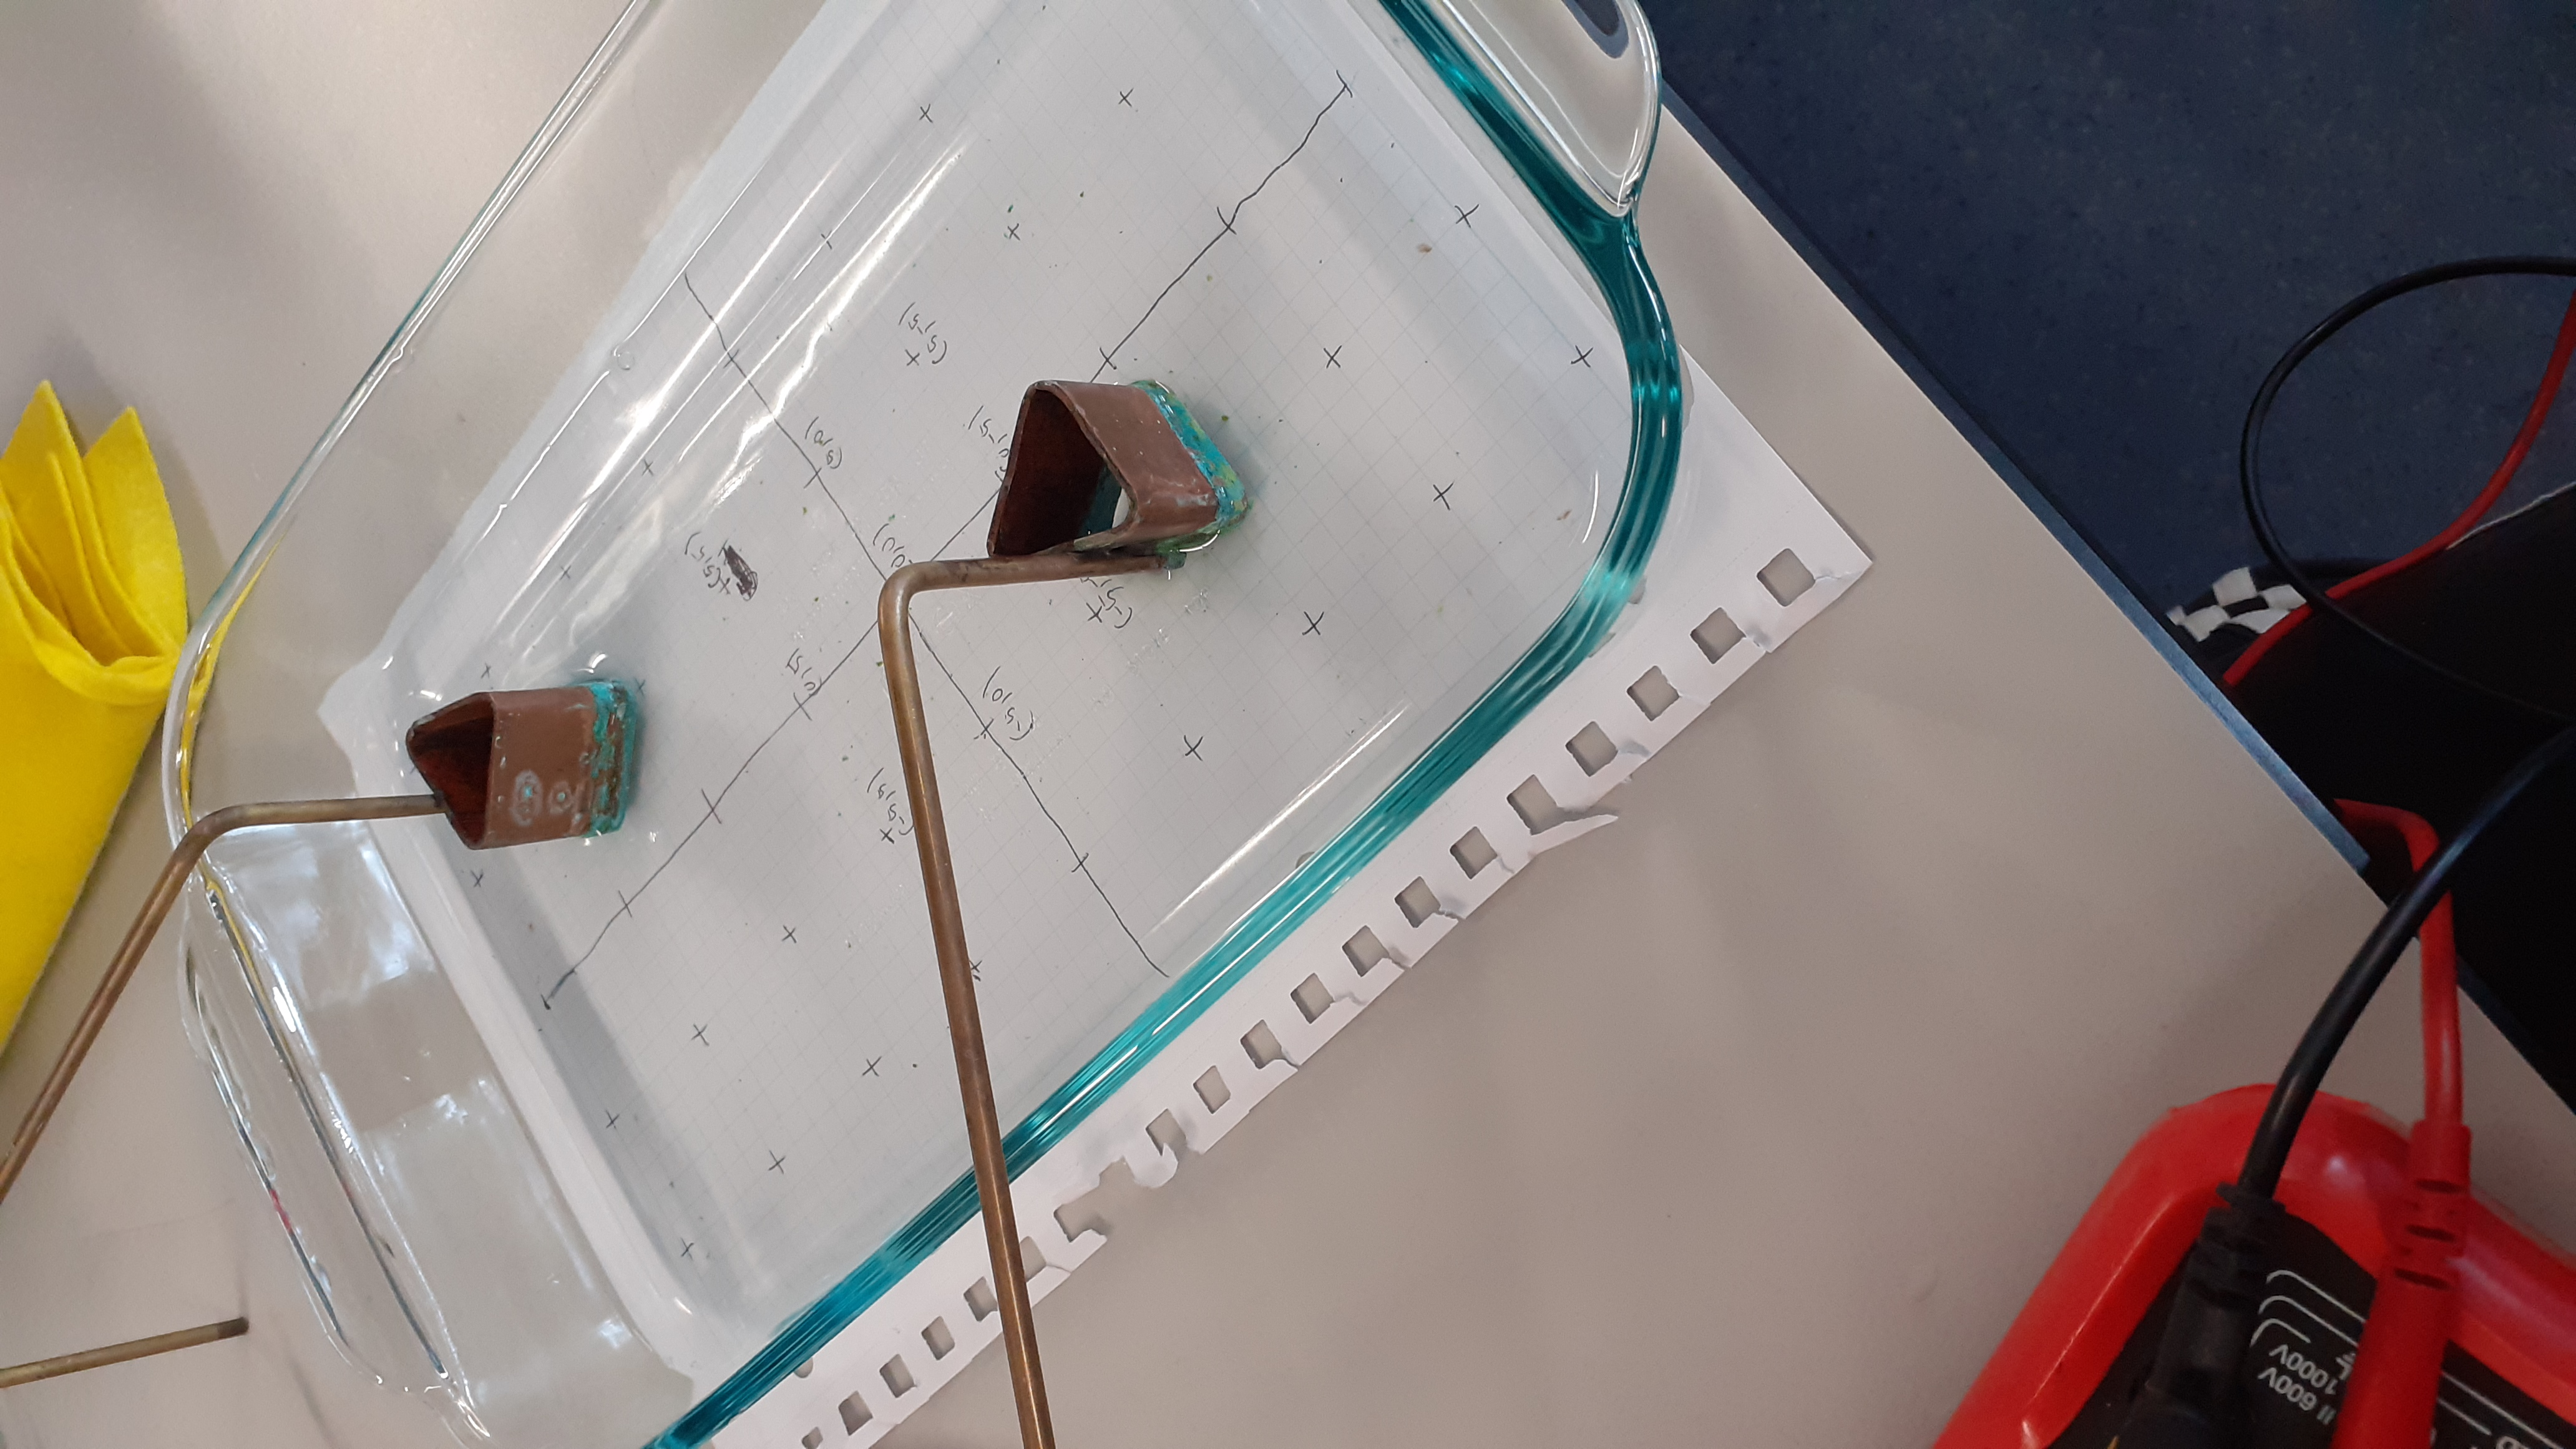
\includegraphics[width=0.8\linewidth, angle=-90]{20190917_152938}
\end{figure}
\subsection{ERRORES}%
\subsection{COMENTARIOS Y OBSERVACIONES}%
Mi primera hoja con ejes estaba mal dibujada y tuve que volver a hacerla.
No puede hallar las lineas de campo en mi primera medición
así que tuve que hacerlo otra vez.

\section{EXPERIENCIA B}
Gravé con mi celular a un multímetro que medía el voltaje de un capacitor.

\subsection{PROCEDIMIENTO Y ANÁLISIS}%
\subsection{ERRORES}%
\subsection{COMENTARIOS Y OBSERVACIONES}%

\begin{figure}[H]
	\centering
	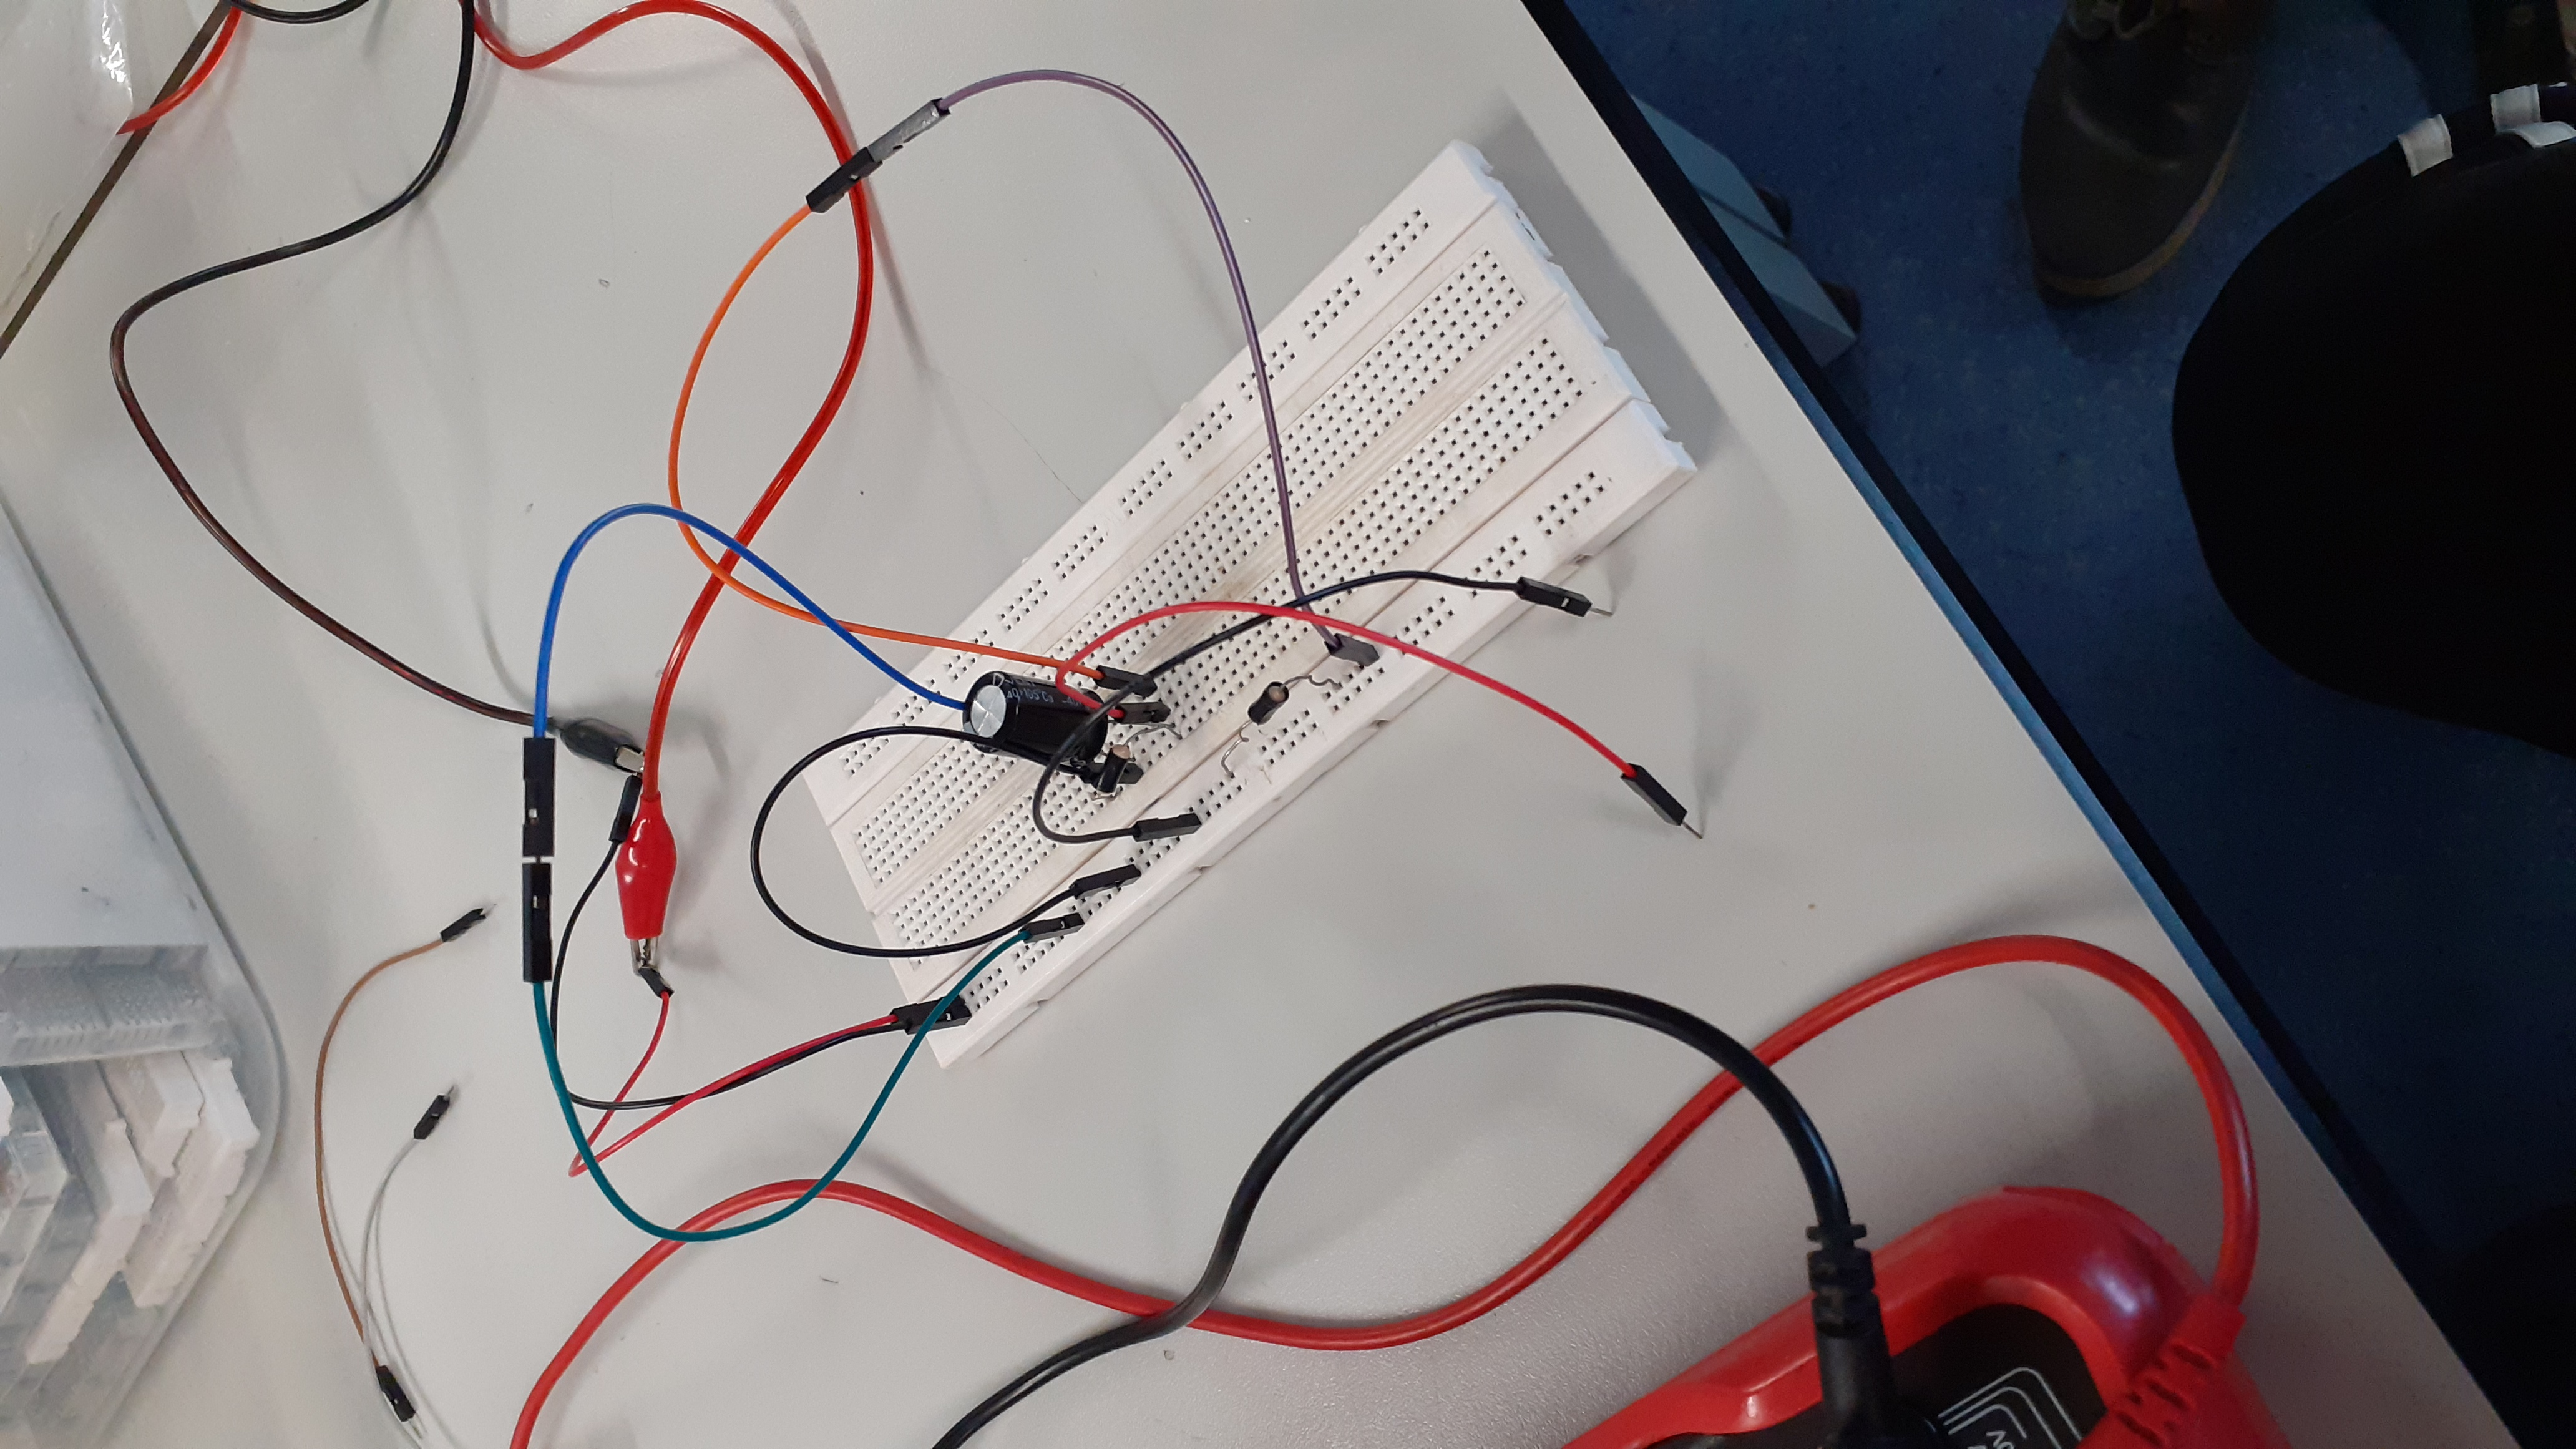
\includegraphics[width=0.8\linewidth, angle=-90]{20190917_163108}
\end{figure}

\section{EXPERIENCIA C}
Medí el campo magnético dentro de una bobina, de dos bobinas y fuera de las bobinas.
Y escribí el promedio en una hoja.

\subsection{PROCEDIMIENTO Y ANÁLISIS}%
\subsection{ERRORES}%
\subsection{COMENTARIOS Y OBSERVACIONES}%
Olvidé medir el radio de la bobina y tomar una foto.

\section{PREGUNTAS DEL CUESTIONARIO}
\subsection{Observación de superficies equipotenciales y líneas de campo eléctrico}
\begin{enumerate}[label=\roman*.]
	\item Dibujar las líneas de campo y las líneas equipotenciales en la hoja cuadriculada,
		no olvidar de dibujar el contorno y la posición de los electrodos usados.
	\item Aproximar la carga de los electrodos al centro de los mismos,
		mostrar el cálculo para obtener la carga total del electrodo.
	\item Escoger 3 puntos que pertenecen a las líneas equipotenciales dibujadas y aproximar el valor
		de la intensidad de campo eléctrico(mostrar los cálculos)
		y también mostrar la dirección aproximada del vector intensidad de campo eléctrico.
\end{enumerate}

\subsection{Carga y descarga de un condensador}
\begin{enumerate}[label=\roman*.]
	\item Mostrar y resolver la ecuación diferencial obtenida al aplicar las leyes de Kirchhoffen un circuito $RC$.
		Mostrar la ecuación de voltaje respecto a tiempo que se debería obtener de manera teórica.
	\item Comparar las funciones de carga y descarga observadas con las funciones obtenidas en el ítem anterior.
		Usar Excel u otra herramienta para realizar la comparación de  las funciones.
	\item Aproximar los valores de las resistencias $R_1$ y $R_2$ utilizando las gráficas obtenidas de carga y descarga.
		Utilizar todos los puntos y obtener valores promedio de resistencias.
\end{enumerate}
\subsection{Magnetismo}
\begin{enumerate}[label=\roman*.]
	\item Utilizando las mediciones de campo magnético para una bobina,
		estimar el valor de su número de vueltas $N$.
	\item Utilizando el valor de $N$ hallado en el paso anterior,
		determine el valor teórico del campo en el punto en el que se realizó la medición utilizando dos bobinas.
		Compare esto con el valor medido, y halle el porcentaje de error respecto al valor teórico.
\end{enumerate}
\section{CONCLUSIONES}
\section{REFERENCIAS}

\end{document}
%}}}
